\documentclass[tikz,border=8pt]{standalone}
\usepackage{lmodern}
\usetikzlibrary{arrows.meta,positioning}
\begin{document}
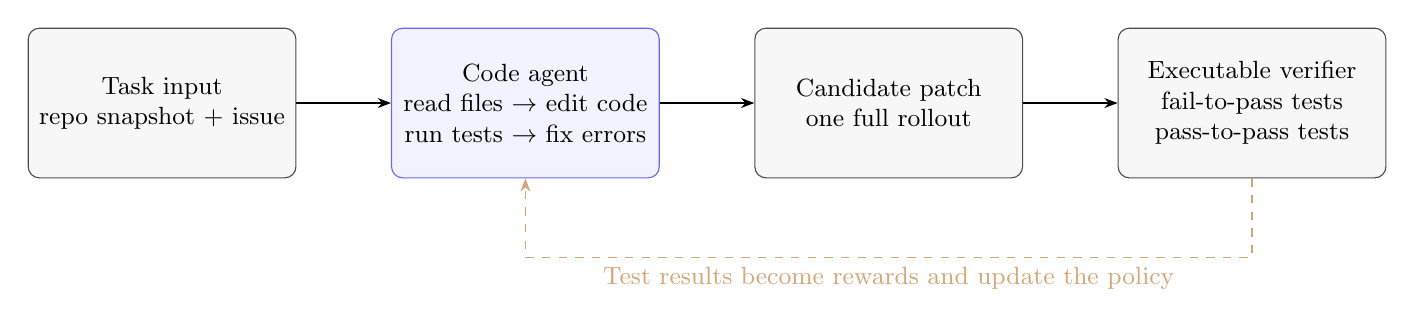
\begin{tikzpicture}[node distance=12mm,>=Stealth,every node/.style={align=center,font=\small},box/.style={rounded corners,draw=black!70,fill=black!3,minimum width=34mm,minimum height=19mm},agent/.style={box,draw=blue!60,fill=blue!5}]
\node[box] (task) {Task input\\repo snapshot + issue};
\node[agent,right=of task] (agent) {Code agent\\read files $\to$ edit code\\run tests $\to$ fix errors};
\node[box,right=of agent] (patch) {Candidate patch\\one full rollout};
\node[box,right=of patch] (verifier) {Executable verifier\\fail-to-pass tests\\pass-to-pass tests};
\draw[->] (task)--(agent); \draw[->] (agent)--(patch); \draw[->] (patch)--(verifier);
\draw[->,dashed,brown!70] (verifier.south) -- ++(0,-10mm) -| node[below,pos=.25]{Test results become rewards and update the policy} (agent.south);
\end{tikzpicture}
\end{document}
